% begin module hyperbolic-functions-def
% % % % % % % % % % % % % % % % % % % % % %
\begin{frame}
The hyperbolic functions satisfy a number of identities that are similar to well-known trigonometric identities.\\
We list some of them here and leave most of the proofs as (easy?) exercises.

\begin{definition}[(some) Hyperbolic Identities]
\[
\begin{array}{l@{\extracolsep{2cm}}l}
\sinh(-x) = -\sinh x & \cosh (-x)=\cosh x\\ [3mm]

\cosh^2(x)-\sinh^x x = 1   & 1-\tanh^2 x = \sech^2 x\\ [3mm]
\end{array}
\]
\[
\sinh(x+y)=\sinh x\cosh y+\cosh x \sinh y
\]
\[
\cosh(x+y)=\cosh x\cosh y+\sinh x \sinh y
\]
\end{definition}




\end{frame}
% % % % % % % % % % % % % % % %
\begin{frame} 
\begin{example}
Prove $\cosh^2x - \sinh^2x = 1$ and $1 - \tanh^2x = \sech^2x$.\\
\textbf{Solution:\\} \pause 
\begin{align*}
\cosh^2x - \sinh^2x & = \left(\frac{e^x+e^{-x}}{2}\right)^2 - \left(\frac{e^x-e^{-x}}{2}\right)^2\\
\onslide<3->{&= \frac{e^2x+2+e^{-2x}}{4}- \frac{e^2x-2+e^{-2x}}{4}}\\
\onslide<4->{& = \frac44 = 1}
\end{align*}
\onslide<5->{For the second identity we use the first to get}
\onslide<6->{
\begin{align*}
\cosh^2x - \sinh^2x = 1 & \;\To\; \frac{\cosh^2x}{\cosh^2x}-\frac{\sinh^2x}{\cosh^2x}= \frac{1}{\cosh^2x}\\
\onslide<7->{&\;\To\; 1 -\tanh^2x = \sech^2x} 
\end{align*}
}

\end{example}
\end{frame}

% % % % % % % % % % % % % % % % % % % % % % % % %
\begin{frame} 
\frametitle{Why ``Hyperbolic Trig"?}

\begin{columns}
\begin{column}{.5\linewidth}
\begin{figure}
\centering
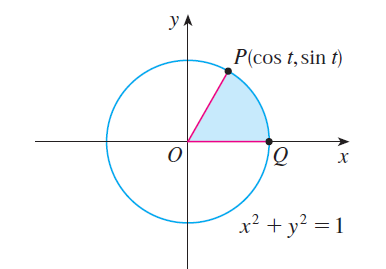
\includegraphics[width=\linewidth]{../../modules/hyperbolic-functions/pictures/trigCircle}
\caption{Trig functions are ``circular": $t$ is the measure of the angle, which (as we know) is equal to twice the area of the shaded circular sector.}
\label{fig:trigCircle}
\end{figure}

\end{column}
\begin{column}{.5\linewidth}
\pause 
\begin{figure}
\centering
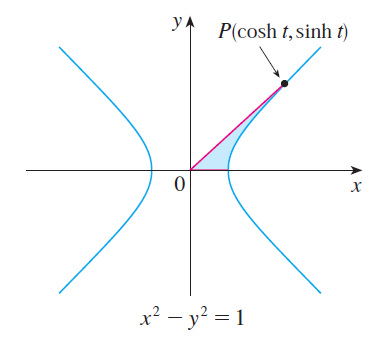
\includegraphics[width=\linewidth]{../../modules/hyperbolic-functions/pictures/hyperbolicSector}
\caption{Here $ t $ represents twice the area of the shaded hyperbolic sector..}
\label{fig:hypCircle}
\end{figure}

\end{column}
\end{columns}

\end{frame}

% end module
